\section{Ejecución de pruebas}
Esta sección detallará todas las pruebas que se han realizado a las distintas propuestas de mejora del sistema. Primero se detallará el entorno de pruebas en el que han sido ejecutadas, con la intención de que sea reproducible, y posteriormente se comentarán los resultados obtenidos.

\subsection{Entorno de pruebas}
Las pruebas han sido realizadas en un entorno JIRA con un proyecto de prueba llamado GPT4, que contiene incidencias ficticias y sobre el proyecto Metaposta Firma Múltiple, un proyecto real de la empresa LKS Next-GobTech, que, en el momento de realización de las pruebas sigue en desarrollo y es actualizado diariamente. El modelo de lenguaje utilizado será GPT-4o, el más avanzado de OpenAI a fecha de realización del trabajo~\cite{gpt4o}. 

\subsection{Evaluación de los resultados}
En cuanto a los resultados, se utilizará el conjunto de 100 preguntas creado durante la realización del trabajo, que contiene una variedad de preguntas de distinta dificultad y con la intención de cubrir la mayor cantidad de casos posibles, se considerará correcta una respuesta si las incidencias devueltas por la API de Jira con la sentencia JQL generada por el modelo son exactamente las mismas que las esperadas, que serán obtenidas mediante otra llamada a la API de Jira con la sentencia JQL predefinida que corresponde a la pregunta.

Los resultados consistirán en una puntuación del 0 al 100, que indicará el número de preguntas respondidas de manera correcta, además, se intentará analiza el por qué de los fallos en las respuestas, si los hubiera, con la intención de mejorar el modelo de lenguaje a futuro.

\subsection{Resultados}
Los resultados obtenidos, evaluados tanto para GPT-4o como para GPT-3.5-turbo se muestran a continuación, en dos gráficas distintas, se muestra el estado inicial, que es la ejecución sin ningún sistema de RAG y las tres propuestas de mejora:

\begin{figure}[H]
    \centering
    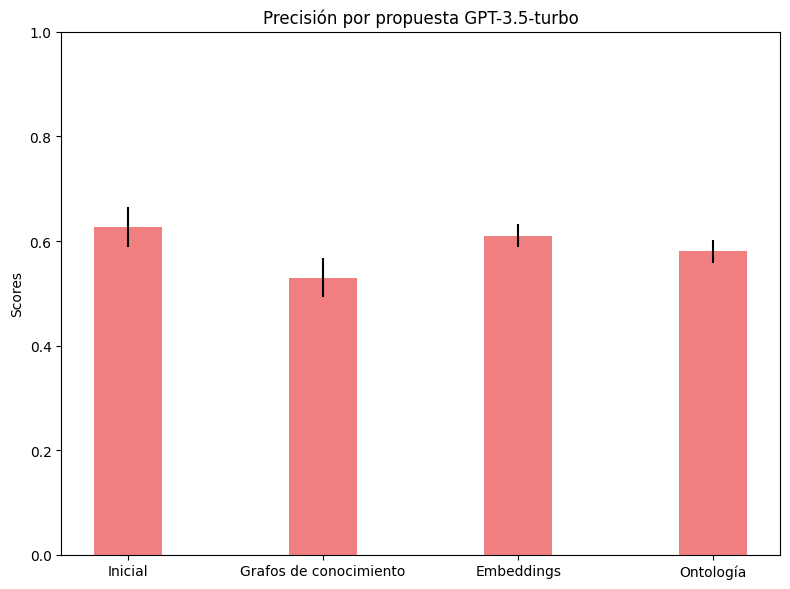
\includegraphics[width=0.8\textwidth]{images/Resultados_gpt35.png}
    \caption{Resultados para GPT-3.5-turbo}
    \label{fig:resultados_gpt35}
\end{figure}

\begin{figure}[H]
    \centering
    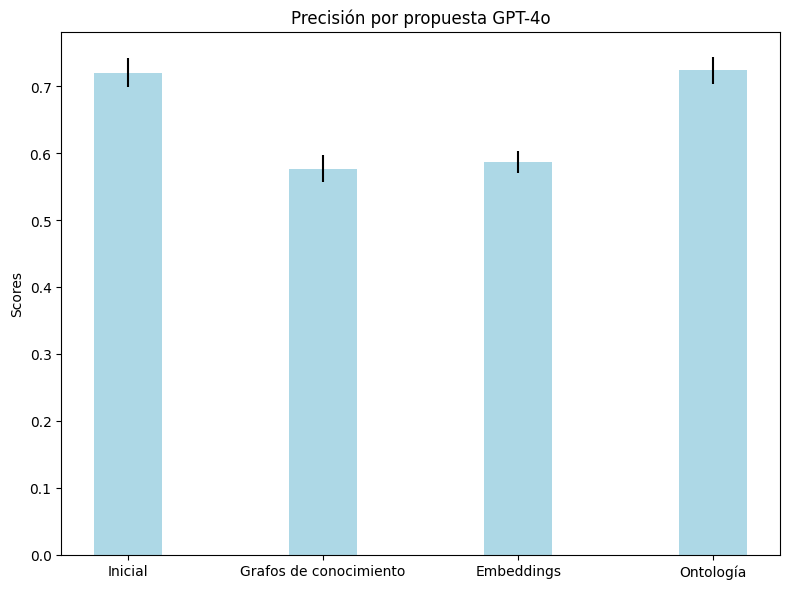
\includegraphics[width=0.8\textwidth]{images/Resultados_gpt4o.png}
    \caption{Resultados para GPT-4o}
    \label{fig:resultados_gpt4o}
\end{figure}